% Generated by Sphinx.
\def\sphinxdocclass{report}
\documentclass[letterpaper,10pt,openany,oneside]{sphinxmanual}
\usepackage[utf8]{inputenc}
\DeclareUnicodeCharacter{00A0}{\nobreakspace}
\usepackage[T1]{fontenc}
\usepackage[english]{babel}
\usepackage{times}
\usepackage[Bjarne]{fncychap}
\usepackage{longtable}
\usepackage{sphinx}
\usepackage{multirow}


\title{Heterogeneous Computing Fundamentals}
\date{July 26, 2012}
\release{}
\author{CSInParallel Project}
\newcommand{\sphinxlogo}{}
\renewcommand{\releasename}{}
\makeindex

\makeatletter
\def\PYG@reset{\let\PYG@it=\relax \let\PYG@bf=\relax%
    \let\PYG@ul=\relax \let\PYG@tc=\relax%
    \let\PYG@bc=\relax \let\PYG@ff=\relax}
\def\PYG@tok#1{\csname PYG@tok@#1\endcsname}
\def\PYG@toks#1+{\ifx\relax#1\empty\else%
    \PYG@tok{#1}\expandafter\PYG@toks\fi}
\def\PYG@do#1{\PYG@bc{\PYG@tc{\PYG@ul{%
    \PYG@it{\PYG@bf{\PYG@ff{#1}}}}}}}
\def\PYG#1#2{\PYG@reset\PYG@toks#1+\relax+\PYG@do{#2}}

\def\PYG@tok@gd{\def\PYG@tc##1{\textcolor[rgb]{0.63,0.00,0.00}{##1}}}
\def\PYG@tok@gu{\let\PYG@bf=\textbf\def\PYG@tc##1{\textcolor[rgb]{0.50,0.00,0.50}{##1}}}
\def\PYG@tok@gt{\def\PYG@tc##1{\textcolor[rgb]{0.00,0.25,0.82}{##1}}}
\def\PYG@tok@gs{\let\PYG@bf=\textbf}
\def\PYG@tok@gr{\def\PYG@tc##1{\textcolor[rgb]{1.00,0.00,0.00}{##1}}}
\def\PYG@tok@cm{\let\PYG@it=\textit\def\PYG@tc##1{\textcolor[rgb]{0.25,0.50,0.56}{##1}}}
\def\PYG@tok@vg{\def\PYG@tc##1{\textcolor[rgb]{0.73,0.38,0.84}{##1}}}
\def\PYG@tok@m{\def\PYG@tc##1{\textcolor[rgb]{0.13,0.50,0.31}{##1}}}
\def\PYG@tok@mh{\def\PYG@tc##1{\textcolor[rgb]{0.13,0.50,0.31}{##1}}}
\def\PYG@tok@cs{\def\PYG@tc##1{\textcolor[rgb]{0.25,0.50,0.56}{##1}}\def\PYG@bc##1{\colorbox[rgb]{1.00,0.94,0.94}{##1}}}
\def\PYG@tok@ge{\let\PYG@it=\textit}
\def\PYG@tok@vc{\def\PYG@tc##1{\textcolor[rgb]{0.73,0.38,0.84}{##1}}}
\def\PYG@tok@il{\def\PYG@tc##1{\textcolor[rgb]{0.13,0.50,0.31}{##1}}}
\def\PYG@tok@go{\def\PYG@tc##1{\textcolor[rgb]{0.19,0.19,0.19}{##1}}}
\def\PYG@tok@cp{\def\PYG@tc##1{\textcolor[rgb]{0.00,0.44,0.13}{##1}}}
\def\PYG@tok@gi{\def\PYG@tc##1{\textcolor[rgb]{0.00,0.63,0.00}{##1}}}
\def\PYG@tok@gh{\let\PYG@bf=\textbf\def\PYG@tc##1{\textcolor[rgb]{0.00,0.00,0.50}{##1}}}
\def\PYG@tok@ni{\let\PYG@bf=\textbf\def\PYG@tc##1{\textcolor[rgb]{0.84,0.33,0.22}{##1}}}
\def\PYG@tok@nl{\let\PYG@bf=\textbf\def\PYG@tc##1{\textcolor[rgb]{0.00,0.13,0.44}{##1}}}
\def\PYG@tok@nn{\let\PYG@bf=\textbf\def\PYG@tc##1{\textcolor[rgb]{0.05,0.52,0.71}{##1}}}
\def\PYG@tok@no{\def\PYG@tc##1{\textcolor[rgb]{0.38,0.68,0.84}{##1}}}
\def\PYG@tok@na{\def\PYG@tc##1{\textcolor[rgb]{0.25,0.44,0.63}{##1}}}
\def\PYG@tok@nb{\def\PYG@tc##1{\textcolor[rgb]{0.00,0.44,0.13}{##1}}}
\def\PYG@tok@nc{\let\PYG@bf=\textbf\def\PYG@tc##1{\textcolor[rgb]{0.05,0.52,0.71}{##1}}}
\def\PYG@tok@nd{\let\PYG@bf=\textbf\def\PYG@tc##1{\textcolor[rgb]{0.33,0.33,0.33}{##1}}}
\def\PYG@tok@ne{\def\PYG@tc##1{\textcolor[rgb]{0.00,0.44,0.13}{##1}}}
\def\PYG@tok@nf{\def\PYG@tc##1{\textcolor[rgb]{0.02,0.16,0.49}{##1}}}
\def\PYG@tok@si{\let\PYG@it=\textit\def\PYG@tc##1{\textcolor[rgb]{0.44,0.63,0.82}{##1}}}
\def\PYG@tok@s2{\def\PYG@tc##1{\textcolor[rgb]{0.25,0.44,0.63}{##1}}}
\def\PYG@tok@vi{\def\PYG@tc##1{\textcolor[rgb]{0.73,0.38,0.84}{##1}}}
\def\PYG@tok@nt{\let\PYG@bf=\textbf\def\PYG@tc##1{\textcolor[rgb]{0.02,0.16,0.45}{##1}}}
\def\PYG@tok@nv{\def\PYG@tc##1{\textcolor[rgb]{0.73,0.38,0.84}{##1}}}
\def\PYG@tok@s1{\def\PYG@tc##1{\textcolor[rgb]{0.25,0.44,0.63}{##1}}}
\def\PYG@tok@gp{\let\PYG@bf=\textbf\def\PYG@tc##1{\textcolor[rgb]{0.78,0.36,0.04}{##1}}}
\def\PYG@tok@sh{\def\PYG@tc##1{\textcolor[rgb]{0.25,0.44,0.63}{##1}}}
\def\PYG@tok@ow{\let\PYG@bf=\textbf\def\PYG@tc##1{\textcolor[rgb]{0.00,0.44,0.13}{##1}}}
\def\PYG@tok@sx{\def\PYG@tc##1{\textcolor[rgb]{0.78,0.36,0.04}{##1}}}
\def\PYG@tok@bp{\def\PYG@tc##1{\textcolor[rgb]{0.00,0.44,0.13}{##1}}}
\def\PYG@tok@c1{\let\PYG@it=\textit\def\PYG@tc##1{\textcolor[rgb]{0.25,0.50,0.56}{##1}}}
\def\PYG@tok@kc{\let\PYG@bf=\textbf\def\PYG@tc##1{\textcolor[rgb]{0.00,0.44,0.13}{##1}}}
\def\PYG@tok@c{\let\PYG@it=\textit\def\PYG@tc##1{\textcolor[rgb]{0.25,0.50,0.56}{##1}}}
\def\PYG@tok@mf{\def\PYG@tc##1{\textcolor[rgb]{0.13,0.50,0.31}{##1}}}
\def\PYG@tok@err{\def\PYG@bc##1{\fcolorbox[rgb]{1.00,0.00,0.00}{1,1,1}{##1}}}
\def\PYG@tok@kd{\let\PYG@bf=\textbf\def\PYG@tc##1{\textcolor[rgb]{0.00,0.44,0.13}{##1}}}
\def\PYG@tok@ss{\def\PYG@tc##1{\textcolor[rgb]{0.32,0.47,0.09}{##1}}}
\def\PYG@tok@sr{\def\PYG@tc##1{\textcolor[rgb]{0.14,0.33,0.53}{##1}}}
\def\PYG@tok@mo{\def\PYG@tc##1{\textcolor[rgb]{0.13,0.50,0.31}{##1}}}
\def\PYG@tok@mi{\def\PYG@tc##1{\textcolor[rgb]{0.13,0.50,0.31}{##1}}}
\def\PYG@tok@kn{\let\PYG@bf=\textbf\def\PYG@tc##1{\textcolor[rgb]{0.00,0.44,0.13}{##1}}}
\def\PYG@tok@o{\def\PYG@tc##1{\textcolor[rgb]{0.40,0.40,0.40}{##1}}}
\def\PYG@tok@kr{\let\PYG@bf=\textbf\def\PYG@tc##1{\textcolor[rgb]{0.00,0.44,0.13}{##1}}}
\def\PYG@tok@s{\def\PYG@tc##1{\textcolor[rgb]{0.25,0.44,0.63}{##1}}}
\def\PYG@tok@kp{\def\PYG@tc##1{\textcolor[rgb]{0.00,0.44,0.13}{##1}}}
\def\PYG@tok@w{\def\PYG@tc##1{\textcolor[rgb]{0.73,0.73,0.73}{##1}}}
\def\PYG@tok@kt{\def\PYG@tc##1{\textcolor[rgb]{0.56,0.13,0.00}{##1}}}
\def\PYG@tok@sc{\def\PYG@tc##1{\textcolor[rgb]{0.25,0.44,0.63}{##1}}}
\def\PYG@tok@sb{\def\PYG@tc##1{\textcolor[rgb]{0.25,0.44,0.63}{##1}}}
\def\PYG@tok@k{\let\PYG@bf=\textbf\def\PYG@tc##1{\textcolor[rgb]{0.00,0.44,0.13}{##1}}}
\def\PYG@tok@se{\let\PYG@bf=\textbf\def\PYG@tc##1{\textcolor[rgb]{0.25,0.44,0.63}{##1}}}
\def\PYG@tok@sd{\let\PYG@it=\textit\def\PYG@tc##1{\textcolor[rgb]{0.25,0.44,0.63}{##1}}}

\def\PYGZbs{\char`\\}
\def\PYGZus{\char`\_}
\def\PYGZob{\char`\{}
\def\PYGZcb{\char`\}}
\def\PYGZca{\char`\^}
% for compatibility with earlier versions
\def\PYGZat{@}
\def\PYGZlb{[}
\def\PYGZrb{]}
\makeatother

\begin{document}

\maketitle
\tableofcontents
\phantomsection\label{index::doc}


Contents:


\chapter{Prerequisites}
\label{Prerequisites/Prerequisites:prerequisites}\label{Prerequisites/Prerequisites:heterogeneous-computing-fundamentals}\label{Prerequisites/Prerequisites::doc}
Before getting started with this module, please keep in mind that we assume you have \textbf{sufficient knowledge with C programming with Message Passing Interface(MPI) and CUDA C.} If you are not familiar with MPI or CUDA C, please read the \textbf{GPU Computing module}, and \textbf{Distributed Memory Computing module}.


\chapter{Introduction to Heterogeneous Computing}
\label{IntroHeterogeneous/IntroHeterogeneous::doc}\label{IntroHeterogeneous/IntroHeterogeneous:introduction-to-heterogeneous-computing}
You have already seen that you can decompose the task and distribute each smaller task to each worker, and let each node work simultaneously in an MPI program. Thus, it enables a programmer to work on a larger problem size, and reduce the computational time. Similarly, CUDA C is a GPU programming language, and is another parallel programming model. Our goal of this module is to program in the hybrid environment CUDA and MPI.

It turns out that we can produce a new parallel programming model that combines MPI and CUDA together. The idea is that we use MPI to distribute work among nodes, each of which uses CUDA to work on its task. In order for this to work, we need to keep in mind that we need to have a cluster or something similar, where each node contains GPUs capable of doing CUDA computation.

{\hfill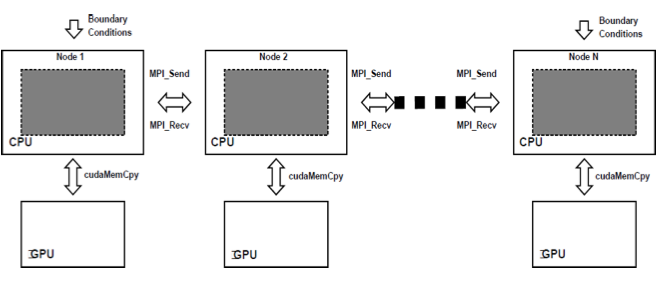
\includegraphics{cudampi.png}\hfill}

\begin{center}Figure 1: Heterogeneous Programming Model: CUDA and MPI from cacuda.googlecode.com {[}1{]}
\end{center}
\begin{notice}{note}{Todo}

Please Do Your Reading: \href{http://www.hipc.org/hipc2009/documents/HIPCSS09Papers/1569247597.pdf}{On the Comparative Performance of Parallel Algorithms on Small GPU/CUDA Clusters}
\end{notice}
\paragraph{References}

{[}1{]} \href{http://cacuda.googlecode.com/files/CaCUDA.pdf}{http://cacuda.googlecode.com/files/CaCUDA.pdf}


\chapter{Coding and Compiling a Heterogeneous Program}
\label{CodingAndCompiling/CodingAndCompiling:coding-and-compiling-a-heterogeneous-program}\label{CodingAndCompiling/CodingAndCompiling::doc}

\section{Heterogeneous Program: Hello World}
\label{CodingAndCompiling/CodingAndCompiling:heterogeneous-program-hello-world}
Distributed memory computing and GPU computing are two different parallel programming models. In this section, you will learn how to put these two parallel models together, and that will speed up your running time. In order to introduce you to this new concept, we will look at the \textbf{Hello World} program using hybrid CUDA and MPI model. In order to combine CUDA and MPI, we need to get their codes to communicate to each other during the compilation. Let's look at the \textbf{Hello World} program below.

\textbf{CUDA program}

\begin{Verbatim}[commandchars=\\\{\},numbers=left,firstnumber=1,stepnumber=1]
\PYG{c+cp}{\#}\PYG{c+cp}{include \textless{}stdio.h\textgreater{}}
\PYG{c+cp}{\#}\PYG{c+cp}{include \textless{}cuda.h\textgreater{}}

\PYG{c+cm}{/* kernel function for GPU */}
\PYG{n}{\PYGZus{}\PYGZus{}global\PYGZus{}\PYGZus{}} \PYG{k+kt}{void} \PYG{n+nf}{kernel}\PYG{p}{(}\PYG{k+kt}{void}\PYG{p}{)} \PYG{p}{\PYGZob{}}
\PYG{p}{\PYGZcb{}}

\PYG{k}{extern} \PYG{l+s}{"}\PYG{l+s}{C}\PYG{l+s}{"} \PYG{k+kt}{void} \PYG{n}{hello}\PYG{p}{(}\PYG{k+kt}{void}\PYG{p}{)} \PYG{p}{\PYGZob{}}
    \PYG{n}{kernel}\PYG{o}{\textless{}}\PYG{o}{\textless{}}\PYG{o}{\textless{}}\PYG{l+m+mi}{1}\PYG{p}{,} \PYG{l+m+mi}{1}\PYG{o}{\textgreater{}}\PYG{o}{\textgreater{}}\PYG{o}{\textgreater{}}\PYG{p}{(}\PYG{p}{)}\PYG{p}{;}
    \PYG{n}{printf}\PYG{p}{(}\PYG{l+s}{"}\PYG{l+s}{Hello World !}\PYG{l+s+se}{\PYGZbs{}n}\PYG{l+s}{"}\PYG{p}{)}\PYG{p}{;}
\PYG{p}{\PYGZcb{}}
\end{Verbatim}

\textbf{MPI program integrated with CUDA}

\begin{Verbatim}[commandchars=\\\{\},numbers=left,firstnumber=1,stepnumber=1]
\PYG{c+cp}{\#}\PYG{c+cp}{include \textless{}mpi.h\textgreater{}}

\PYG{c+cp}{\#}\PYG{c+cp}{define MAX 80    }\PYG{c+cm}{/* maximum characters for naming the node */}

\PYG{c+cm}{/* Declaring the CUDA function */}
\PYG{k+kt}{void} \PYG{n}{hello}\PYG{p}{(}\PYG{p}{)}\PYG{p}{;}

\PYG{k+kt}{int} \PYG{n+nf}{main}\PYG{p}{(}\PYG{k+kt}{int} \PYG{n}{argc}\PYG{p}{,} \PYG{k+kt}{char} \PYG{o}{*}\PYG{n}{argv}\PYG{p}{[}\PYG{p}{]}\PYG{p}{)} \PYG{p}{\PYGZob{}}

   \PYG{k+kt}{int} \PYG{n}{rank}\PYG{p}{,} \PYG{n}{nprocs}\PYG{p}{,} \PYG{n}{len}\PYG{p}{;}
   \PYG{k+kt}{char} \PYG{n}{name}\PYG{p}{[}\PYG{n}{MAX}\PYG{p}{]}\PYG{p}{;}      \PYG{c+cm}{/* char array for storing the name of each node */}

   \PYG{c+cm}{/* Initializing the MPI execution environment */}
   \PYG{n}{MPI\PYGZus{}Init}\PYG{p}{(}\PYG{o}{\&}\PYG{n}{argc}\PYG{p}{,} \PYG{o}{\&}\PYG{n}{argv}\PYG{p}{)}\PYG{p}{;}
   \PYG{n}{MPI\PYGZus{}Comm\PYGZus{}rank}\PYG{p}{(}\PYG{n}{MPI\PYGZus{}COMM\PYGZus{}WORLD}\PYG{p}{,} \PYG{o}{\&}\PYG{n}{rank}\PYG{p}{)}\PYG{p}{;}
   \PYG{n}{MPI\PYGZus{}Comm\PYGZus{}size}\PYG{p}{(}\PYG{n}{MPI\PYGZus{}COMM\PYGZus{}WORLD}\PYG{p}{,} \PYG{o}{\&}\PYG{n}{size}\PYG{p}{)}\PYG{p}{;}
   \PYG{n}{MPI\PYGZus{}Get\PYGZus{}processor\PYGZus{}name}\PYG{p}{(}\PYG{n}{name}\PYG{p}{,} \PYG{o}{\&}\PYG{n}{len}\PYG{p}{)}\PYG{p}{;}

   \PYG{c+cm}{/* Call CUDA function */}
   \PYG{n}{hello}\PYG{p}{(}\PYG{p}{)}\PYG{p}{;}

   \PYG{c+cm}{/* Print the rank, size, and name of each node */}
   \PYG{n}{printf}\PYG{p}{(}\PYG{l+s}{"}\PYG{l+s}{I am \%d of \%d on \%s}\PYG{l+s+se}{\PYGZbs{}n}\PYG{l+s}{"}\PYG{p}{,} \PYG{n}{rank}\PYG{p}{,} \PYG{n}{size}\PYG{p}{,} \PYG{n}{name}\PYG{p}{)}\PYG{p}{;}

   \PYG{c+cm}{/*Terminating the MPI environment*/}
   \PYG{n}{MPI\PYGZus{}Finalize}\PYG{p}{(}\PYG{p}{)}\PYG{p}{;}
   \PYG{k}{return} \PYG{l+m+mi}{0}\PYG{p}{;}
\PYG{p}{\PYGZcb{}}
\end{Verbatim}
\begin{quote}\begin{description}
\item[{Comments}] \leavevmode\begin{itemize}
\item {} 
From source codes above, CUDA program creates a grid consisting a block, which has a single thread. It will print “Hello World !”. The \textbf{hello} function in CUDA program uses the keyword \textbf{extern “C”}, so the MPI program is able to link to use \textbf{hello} function using a `C' compatible header file that contains just the declaration of \textbf{hello} function. In addition, MPI program only creates the MPI execution environment, defines the size of the MPI\_COMM\_WORLD, gives the unique rank to each process, calls \textbf{hello} function from CUDA program to print ``Hello World !'', and prints the rank, size, and name of the process. Finally, all processes terminate the MPI execution environment.

\end{itemize}

\end{description}\end{quote}


\section{Compiling a Heterogeneous Program}
\label{CodingAndCompiling/CodingAndCompiling:compiling-a-heterogeneous-program}
The most common way of compiling a heterogeneous program MPI and Cuda is:
\begin{enumerate}
\item {} 
Make a CUDA object from the CUDA program. This can be done by using this command on the terminal:

\begin{Verbatim}[commandchars=\\\{\}]
\PYG{n}{nvcc} \PYG{o}{-}\PYG{n}{c} \PYG{n}{cuda}\PYG{p}{.}\PYG{n}{cu} \PYG{o}{-}\PYG{n}{o} \PYG{n}{cuda}\PYG{p}{.}\PYG{n}{o}
\end{Verbatim}

\item {} 
Make an MPI object from MPI program. This can be done by using this command on the terminal:

\begin{Verbatim}[commandchars=\\\{\}]
\PYG{n}{mpicc} \PYG{o}{-}\PYG{n}{c} \PYG{n}{mpi}\PYG{p}{.}\PYG{n}{c} \PYG{o}{-}\PYG{n}{o} \PYG{n}{mpi}\PYG{p}{.}\PYG{n}{o}
\end{Verbatim}

\item {} 
Make an executable file from both objects. This can be done by using this command on the terminal:

\begin{Verbatim}[commandchars=\\\{\}]
\PYG{n}{mpicc} \PYG{o}{-}\PYG{n}{o} \PYG{n}{cudampi} \PYG{n}{mpi}\PYG{p}{.}\PYG{n}{o} \PYG{n}{cuda}\PYG{p}{.}\PYG{n}{o} \PYG{o}{-}\PYG{n}{L}\PYG{o}{/}\PYG{n}{usr}\PYG{o}{/}\PYG{n}{local}\PYG{o}{/}\PYG{n}{cuda}\PYG{o}{/}\PYG{n}{lib64} \PYG{o}{-}\PYG{n}{lcudart}
\end{Verbatim}

\end{enumerate}

To execute the executable file, \textbf{cudampi}, we can enter the following command on the terminal:

\begin{Verbatim}[commandchars=\\\{\}]
mpirun -machinefile machines -x LD\_LIBRARY\_PATH -np \#processes ./cudampi
\end{Verbatim}


\subsection{Timing a Heterogeneous CUDA and MPI}
\label{CodingAndCompiling/CodingAndCompiling:timing-a-heterogeneous-cuda-and-mpi}\begin{itemize}
\item {} 
In order to time your hybrid CUDA and MPI program, you just need to use MPI\_Wtime() function as in an MPI program.

\item {} 
We need to keep in mind that a heterogeneous CUDA and MPI program theoretically has lower running time than an MPI does; however, running time also depends on each node's properties such as memory. Copying data from a CPU to GPU may take a long period of time, which results in a much longer running time for a heterogeneous program. Therefore, you do not always get benefits from the heterogeneous programming model.

\end{itemize}


\subsection{Activity 1: Vector Addition}
\label{CodingAndCompiling/CodingAndCompiling:activity-1-vector-addition}
In this activity, we are going to compute vector addition by using hybrid programming model, CUDA and MPI. Vector addition is very simple and easy. Suppose we have vector \emph{A} and vector \emph{B}, and both have the same length. To add vector \emph{A} and \emph{B}, we just add the corresponding elements of \emph{A} and \emph{B}. This results a new vector of the same length.
\begin{quote}\begin{description}
\item[{Comments on CUDA Program}] \leavevmode\begin{itemize}
\item {} 
We will walk you through this first activity step by step. First, let's look at the CUDA program for vector addition. We need to have a kernel function for vector addition. This should be straight forward to you. Each thread computes an element of the result matrix, where thread index is the index of that element.

\begin{Verbatim}[commandchars=\\\{\}]
\PYG{n}{\PYGZus{}\PYGZus{}global\PYGZus{}\PYGZus{}} \PYG{k+kt}{void} \PYG{n+nf}{kernel}\PYG{p}{(}\PYG{k+kt}{int} \PYG{o}{*}\PYG{n}{a}\PYG{p}{,} \PYG{k+kt}{int} \PYG{o}{*}\PYG{n}{b}\PYG{p}{,} \PYG{k+kt}{int} \PYG{o}{*}\PYG{n}{c}\PYG{p}{)} \PYG{p}{\PYGZob{}}
        \PYG{c+cm}{/* this thread index is the index of the vector */}
        \PYG{k+kt}{int} \PYG{n}{index} \PYG{o}{=} \PYG{n}{blockIdx}\PYG{p}{.}\PYG{n}{x} \PYG{o}{*} \PYG{n}{blockDim}\PYG{p}{.}\PYG{n}{x} \PYG{o}{+} \PYG{n}{threadIdx}\PYG{p}{.}\PYG{n}{x}\PYG{p}{;}
        \PYG{c+c1}{// TO DO}
        \PYG{c+c1}{// add corresponding elements of a and b}
        \PYG{c+c1}{// end TO DO}
\PYG{p}{\PYGZcb{}}
\end{Verbatim}

\item {} 
Another function in the CUDA program is \textbf{run\_kernel}, which works on the host(CPU) and calls the kernel function on the device(GPU). This function allocates memory on the GPU for storing input vectors, copies input vectors onto the device, does the calculations on the device, copies output vector back to the host, and erases all those vectors on the device. This function will be called in the MPI program.

\begin{Verbatim}[commandchars=\\\{\}]
\PYG{c+cm}{/*}
\PYG{c+cm}{* size is the number of elements in the vector}
\PYG{c+cm}{* nblocks is the number of blocks per grid}
\PYG{c+cm}{* nthreads is the number of threads per block}
\PYG{c+cm}{*/}
\PYG{k}{extern} \PYG{l+s}{"}\PYG{l+s}{C}\PYG{l+s}{"} \PYG{k+kt}{void} \PYG{n}{run\PYGZus{}kernel}\PYG{p}{(}\PYG{k+kt}{int} \PYG{o}{*}\PYG{n}{a}\PYG{p}{,} \PYG{k+kt}{int} \PYG{o}{*}\PYG{n}{b}\PYG{p}{,} \PYG{k+kt}{int} \PYG{o}{*}\PYG{n}{c}\PYG{p}{,} \PYG{k+kt}{int} \PYG{n}{size}\PYG{p}{,} \PYG{k+kt}{int} \PYG{n}{nblocks}\PYG{p}{,} \PYG{k+kt}{int} \PYG{n}{nthreads}\PYG{p}{)} \PYG{p}{\PYGZob{}}

        \PYG{c+cm}{/* pointers for storing each vector on the device*/}
        \PYG{k+kt}{int} \PYG{o}{*}\PYG{n}{dev\PYGZus{}a}\PYG{p}{,} \PYG{o}{*}\PYG{n}{dev\PYGZus{}b}\PYG{p}{,} \PYG{o}{*}\PYG{n}{dev\PYGZus{}c}\PYG{p}{;}

        \PYG{c+cm}{/* Allocate memory on the device */}
        \PYG{n}{cudaMalloc}\PYG{p}{(}\PYG{p}{(}\PYG{k+kt}{void}\PYG{o}{*}\PYG{o}{*}\PYG{p}{)}\PYG{o}{\&}\PYG{n}{dev\PYGZus{}a}\PYG{p}{,} \PYG{k}{sizeof}\PYG{p}{(}\PYG{k+kt}{int}\PYG{p}{)}\PYG{o}{*}\PYG{n}{size}\PYG{p}{)}\PYG{p}{;}
        \PYG{n}{cudaMalloc}\PYG{p}{(}\PYG{p}{(}\PYG{k+kt}{void}\PYG{o}{*}\PYG{o}{*}\PYG{p}{)}\PYG{o}{\&}\PYG{n}{dev\PYGZus{}b}\PYG{p}{,} \PYG{k}{sizeof}\PYG{p}{(}\PYG{k+kt}{int}\PYG{p}{)}\PYG{o}{*}\PYG{n}{size}\PYG{p}{)}\PYG{p}{;}
        \PYG{n}{cudaMalloc}\PYG{p}{(}\PYG{p}{(}\PYG{k+kt}{void}\PYG{o}{*}\PYG{o}{*}\PYG{p}{)}\PYG{o}{\&}\PYG{n}{dev\PYGZus{}c}\PYG{p}{,} \PYG{k}{sizeof}\PYG{p}{(}\PYG{k+kt}{int}\PYG{p}{)}\PYG{o}{*}\PYG{n}{size}\PYG{p}{)}\PYG{p}{;}

        \PYG{c+cm}{/* Copy vectors a and b from host to device */}
        \PYG{n}{cudaMemcpy}\PYG{p}{(}\PYG{n}{dev\PYGZus{}a}\PYG{p}{,} \PYG{n}{a}\PYG{p}{,} \PYG{k}{sizeof}\PYG{p}{(}\PYG{k+kt}{int}\PYG{p}{)}\PYG{o}{*}\PYG{n}{size}\PYG{p}{,} \PYG{n}{cudaMemcpyHostToDevice}\PYG{p}{)}\PYG{p}{;}
        \PYG{n}{cudaMemcpy}\PYG{p}{(}\PYG{n}{dev\PYGZus{}b}\PYG{p}{,} \PYG{n}{b}\PYG{p}{,} \PYG{k}{sizeof}\PYG{p}{(}\PYG{k+kt}{int}\PYG{p}{)}\PYG{o}{*}\PYG{n}{size}\PYG{p}{,} \PYG{n}{cudaMemcpyHostToDevice}\PYG{p}{)}\PYG{p}{;}

        \PYG{c+cm}{/* Calling the kernel function to do calculation */}

        \PYG{c+c1}{// TO DO}
        \PYG{c+c1}{// Call kernel function here}
        \PYG{c+c1}{// end TO DO}

        \PYG{c+cm}{/* Copy the result vector from device to host*/}
        \PYG{n}{cudaMemcpy}\PYG{p}{(}\PYG{n}{c}\PYG{p}{,} \PYG{n}{dev\PYGZus{}c}\PYG{p}{,} \PYG{k}{sizeof}\PYG{p}{(}\PYG{k+kt}{int}\PYG{p}{)}\PYG{o}{*}\PYG{n}{size}\PYG{p}{,} \PYG{n}{cudaMemcpyDeviceToHost}\PYG{p}{)}\PYG{p}{;}

        \PYG{c+cm}{/* Free memory on the device */}
        \PYG{n}{cudaFree}\PYG{p}{(}\PYG{n}{dev\PYGZus{}a}\PYG{p}{)}\PYG{p}{;}
        \PYG{n}{cudaFree}\PYG{p}{(}\PYG{n}{dev\PYGZus{}b}\PYG{p}{)}\PYG{p}{;}
        \PYG{n}{cudaFree}\PYG{p}{(}\PYG{n}{dev\PYGZus{}c}\PYG{p}{)}\PYG{p}{;}
\PYG{p}{\PYGZcb{}}
\end{Verbatim}

\end{itemize}

\item[{Comments on MPI Program}] \leavevmode\begin{itemize}
\item {} 
This MPI program is basically the MPI program with an addition of a function from CUDA program. It splits both input vectors into smaller pieces, and sends each piece of each vector to each worker. Then we will call the \textbf{run\_kernel} function from CUDA program to calculate additions of the two vectors on each node.

\item {} 
First we need to initialize the MPI execution environment, define the size of all processes, and give a unique rank to each process. Then we will ask the master to initialize the input vectors, split the input vectors into smaller chunks, and send these chunks to each process. Your task is to send the pieces of input vectors to each worker.

\begin{Verbatim}[commandchars=\\\{\}]
\PYG{c+cm}{/******************** Master ***********************/}
\PYG{k}{if} \PYG{p}{(}\PYG{n}{rank} \PYG{o}{=}\PYG{o}{=} \PYG{n}{MASTER}\PYG{p}{)} \PYG{p}{\PYGZob{}}
        \PYG{c+cm}{/* Initializing both vectors in master */}
        \PYG{k+kt}{int} \PYG{n}{sum} \PYG{o}{=} \PYG{l+m+mi}{0}\PYG{p}{;}
        \PYG{k}{for} \PYG{p}{(}\PYG{n}{i} \PYG{o}{=} \PYG{l+m+mi}{0}\PYG{p}{;} \PYG{n}{i} \PYG{o}{\textless{}} \PYG{n}{WIDTH}\PYG{p}{;} \PYG{n}{i}\PYG{o}{+}\PYG{o}{+}\PYG{p}{)} \PYG{p}{\PYGZob{}}
                \PYG{n}{arr\PYGZus{}a}\PYG{p}{[}\PYG{n}{i}\PYG{p}{]} \PYG{o}{=} \PYG{n}{i}\PYG{p}{;}
                \PYG{n}{arr\PYGZus{}b}\PYG{p}{[}\PYG{n}{i}\PYG{p}{]} \PYG{o}{=} \PYG{n}{i}\PYG{o}{*}\PYG{n}{i}\PYG{p}{;}
        \PYG{p}{\PYGZcb{}}
        \PYG{c+cm}{/* Decomposing the problem into smaller problems, and send each task}
\PYG{c+cm}{        * to each worker. Master not taking part in any computation.}
\PYG{c+cm}{        */}
        \PYG{n}{num\PYGZus{}worker} \PYG{o}{=} \PYG{n}{size} \PYG{o}{-} \PYG{l+m+mi}{1}\PYG{p}{;}
        \PYG{n}{ave\PYGZus{}size} \PYG{o}{=} \PYG{n}{WIDTH}\PYG{o}{/}\PYG{n}{num\PYGZus{}worker}\PYG{p}{;}    \PYG{c+cm}{/* finding the average size of task for a process */}
        \PYG{n}{extra} \PYG{o}{=} \PYG{n}{WIDTH} \PYG{o}{\%} \PYG{n}{num\PYGZus{}worker}\PYG{p}{;}             \PYG{c+cm}{/* finding extra task for some processes*/}
        \PYG{n}{offset} \PYG{o}{=} \PYG{l+m+mi}{0}\PYG{p}{;}
        \PYG{n}{mtype} \PYG{o}{=} \PYG{n}{FROM\PYGZus{}MASTER}\PYG{p}{;}                    \PYG{c+cm}{/* message sends from master */}

        \PYG{c+cm}{/* Master sends each task to each worker */}
        \PYG{k}{for} \PYG{p}{(}\PYG{n}{dest} \PYG{o}{=} \PYG{l+m+mi}{1}\PYG{p}{;} \PYG{n}{dest} \PYG{o}{\textless{}}\PYG{o}{=} \PYG{n}{num\PYGZus{}worker}\PYG{p}{;} \PYG{n}{dest}\PYG{o}{+}\PYG{o}{+}\PYG{p}{)} \PYG{p}{\PYGZob{}}
                \PYG{n}{eles} \PYG{o}{=} \PYG{p}{(}\PYG{n}{dest} \PYG{o}{\textless{}}\PYG{o}{=} \PYG{n}{extra}\PYG{p}{)} \PYG{o}{?} \PYG{n}{ave\PYGZus{}size} \PYG{o}{+} \PYG{l+m+mi}{1}\PYG{o}{:} \PYG{n}{ave\PYGZus{}size}\PYG{p}{;}
                \PYG{n}{MPI\PYGZus{}Send}\PYG{p}{(}\PYG{o}{\&}\PYG{n}{offset}\PYG{p}{,} \PYG{l+m+mi}{1}\PYG{p}{,} \PYG{n}{MPI\PYGZus{}INT}\PYG{p}{,} \PYG{n}{dest}\PYG{p}{,} \PYG{n}{mtype}\PYG{p}{,} \PYG{n}{MPI\PYGZus{}COMM\PYGZus{}WORLD}\PYG{p}{)}\PYG{p}{;}
                \PYG{n}{MPI\PYGZus{}Send}\PYG{p}{(}\PYG{o}{\&}\PYG{n}{eles}\PYG{p}{,} \PYG{l+m+mi}{1}\PYG{p}{,} \PYG{n}{MPI\PYGZus{}INT}\PYG{p}{,} \PYG{n}{dest}\PYG{p}{,} \PYG{n}{mtype}\PYG{p}{,} \PYG{n}{MPI\PYGZus{}COMM\PYGZus{}WORLD}\PYG{p}{)}\PYG{p}{;}

                \PYG{c+c1}{// TO DO}
                \PYG{c+c1}{// send a piece of each vector to each worker}
                \PYG{c+c1}{// end TO DO}

                \PYG{n}{printf}\PYG{p}{(}\PYG{l+s}{"}\PYG{l+s}{Master sent elements \%d to \%d to rank \%d}\PYG{l+s+se}{\PYGZbs{}n}\PYG{l+s}{"}\PYG{p}{,} \PYG{n}{offset}\PYG{p}{,} \PYG{n}{offset} \PYG{o}{+} \PYG{n}{eles}\PYG{p}{,} \PYG{n}{dest}\PYG{p}{)}\PYG{p}{;}
                \PYG{n}{offset} \PYG{o}{+}\PYG{o}{=} \PYG{n}{eles}\PYG{p}{;}
        \PYG{p}{\PYGZcb{}}
\PYG{p}{\PYGZcb{}}
\end{Verbatim}

\item {} 
Then we want all workers to receive the messages sent from master, and we call the \textbf{run\_kernel} function from CUDA program to compute the sum of both vectors on each worker. This function will call the kernel function and compute additions on the GPU of each worker. When they are done with computations, each worker needs to send its result vector to the master. Your task is to receive the vectors sent from master, and to call \textbf{run\_kernel} function from the CUDA program.

\begin{Verbatim}[commandchars=\\\{\}]
\PYG{c+cm}{/* The workers receive the task from master, and will each run run\PYGZus{}kernel to}
\PYG{c+cm}{* compute the sum of each element from vector a and vector b. After computation}
\PYG{c+cm}{* each worker sends the result back to master node.}
\PYG{c+cm}{*/}
\PYG{c+cm}{/******************************* Workers **************************/}
\PYG{k}{if} \PYG{p}{(}\PYG{n}{rank} \PYG{o}{\textgreater{}} \PYG{n}{MASTER}\PYG{p}{)} \PYG{p}{\PYGZob{}}
        \PYG{n}{mtype} \PYG{o}{=} \PYG{n}{FROM\PYGZus{}MASTER}\PYG{p}{;}
        \PYG{n}{source} \PYG{o}{=} \PYG{n}{MASTER}\PYG{p}{;}
        \PYG{c+cm}{/* Receive data from master */}

        \PYG{c+c1}{// TO DO}
        \PYG{c+c1}{// receive the vectors sent from master}
        \PYG{c+c1}{// end TO DO}

        \PYG{n}{MPI\PYGZus{}Get\PYGZus{}processor\PYGZus{}name}\PYG{p}{(}\PYG{n}{name}\PYG{p}{,} \PYG{o}{\&}\PYG{n}{len}\PYG{p}{)}\PYG{p}{;}

        \PYG{c+cm}{/* Use kernel to compute the sum of element a and b */}

        \PYG{c+c1}{// TO DO}
        \PYG{c+c1}{// call run\PYGZus{}kernel function here}
        \PYG{c+c1}{// end TO DO}

        \PYG{c+cm}{/* send result back to the master */}
        \PYG{n}{mtype} \PYG{o}{=} \PYG{n}{FROM\PYGZus{}WORKER}\PYG{p}{;}
        \PYG{n}{MPI\PYGZus{}Send}\PYG{p}{(}\PYG{o}{\&}\PYG{n}{offset}\PYG{p}{,} \PYG{l+m+mi}{1}\PYG{p}{,} \PYG{n}{MPI\PYGZus{}INT}\PYG{p}{,} \PYG{n}{MASTER}\PYG{p}{,} \PYG{n}{mtype}\PYG{p}{,} \PYG{n}{MPI\PYGZus{}COMM\PYGZus{}WORLD}\PYG{p}{)}\PYG{p}{;}
        \PYG{n}{MPI\PYGZus{}Send}\PYG{p}{(}\PYG{o}{\&}\PYG{n}{eles}\PYG{p}{,} \PYG{l+m+mi}{1}\PYG{p}{,} \PYG{n}{MPI\PYGZus{}INT}\PYG{p}{,} \PYG{n}{MASTER}\PYG{p}{,} \PYG{n}{mtype}\PYG{p}{,} \PYG{n}{MPI\PYGZus{}COMM\PYGZus{}WORLD}\PYG{p}{)}\PYG{p}{;}
        \PYG{n}{MPI\PYGZus{}Send}\PYG{p}{(}\PYG{o}{\&}\PYG{n}{arr\PYGZus{}c}\PYG{p}{,} \PYG{n}{eles}\PYG{p}{,} \PYG{n}{MPI\PYGZus{}INT}\PYG{p}{,} \PYG{n}{MASTER}\PYG{p}{,} \PYG{n}{mtype}\PYG{p}{,} \PYG{n}{MPI\PYGZus{}COMM\PYGZus{}WORLD}\PYG{p}{)}\PYG{p}{;}
\PYG{p}{\PYGZcb{}}
\end{Verbatim}

\item {} 
We need to ask the master to receive the result vector sent from each worker. We then can check to see if they are correct. Verification part should not be included in your timing.

\begin{Verbatim}[commandchars=\\\{\}]
\PYG{c+cm}{/* Master receives the result from each worker */}
\PYG{n}{mtype} \PYG{o}{=} \PYG{n}{FROM\PYGZus{}WORKER}\PYG{p}{;}
\PYG{k}{for}\PYG{p}{(}\PYG{n}{i} \PYG{o}{=} \PYG{l+m+mi}{1}\PYG{p}{;} \PYG{n}{i} \PYG{o}{\textless{}}\PYG{o}{=} \PYG{n}{num\PYGZus{}worker}\PYG{p}{;} \PYG{n}{i}\PYG{o}{+}\PYG{o}{+}\PYG{p}{)} \PYG{p}{\PYGZob{}}
        \PYG{n}{source} \PYG{o}{=} \PYG{n}{i}\PYG{p}{;}
        \PYG{n}{MPI\PYGZus{}Recv}\PYG{p}{(}\PYG{o}{\&}\PYG{n}{offset}\PYG{p}{,} \PYG{l+m+mi}{1}\PYG{p}{,} \PYG{n}{MPI\PYGZus{}INT}\PYG{p}{,} \PYG{n}{source}\PYG{p}{,} \PYG{n}{mtype}\PYG{p}{,} \PYG{n}{MPI\PYGZus{}COMM\PYGZus{}WORLD}\PYG{p}{,} \PYG{o}{\&}\PYG{n}{status}\PYG{p}{)}\PYG{p}{;}
        \PYG{n}{MPI\PYGZus{}Recv}\PYG{p}{(}\PYG{o}{\&}\PYG{n}{eles}\PYG{p}{,} \PYG{l+m+mi}{1}\PYG{p}{,} \PYG{n}{MPI\PYGZus{}INT}\PYG{p}{,} \PYG{n}{source}\PYG{p}{,} \PYG{n}{mtype}\PYG{p}{,} \PYG{n}{MPI\PYGZus{}COMM\PYGZus{}WORLD}\PYG{p}{,} \PYG{o}{\&}\PYG{n}{status}\PYG{p}{)}\PYG{p}{;}
        \PYG{n}{MPI\PYGZus{}Recv}\PYG{p}{(}\PYG{o}{\&}\PYG{n}{arr\PYGZus{}c}\PYG{p}{[}\PYG{n}{offset}\PYG{p}{]}\PYG{p}{,} \PYG{n}{eles}\PYG{p}{,} \PYG{n}{MPI\PYGZus{}INT}\PYG{p}{,} \PYG{n}{source}\PYG{p}{,} \PYG{n}{mtype}\PYG{p}{,} \PYG{n}{MPI\PYGZus{}COMM\PYGZus{}WORLD}\PYG{p}{,} \PYG{o}{\&}\PYG{n}{status}\PYG{p}{)}\PYG{p}{;}
        \PYG{n}{printf}\PYG{p}{(}\PYG{l+s}{"}\PYG{l+s}{Received results from task \%d}\PYG{l+s+se}{\PYGZbs{}n}\PYG{l+s}{"}\PYG{p}{,} \PYG{n}{source}\PYG{p}{)}\PYG{p}{;}
\PYG{p}{\PYGZcb{}}

\PYG{c+cm}{/* checking the result on master */}
\PYG{k}{for} \PYG{p}{(}\PYG{n}{i} \PYG{o}{=} \PYG{l+m+mi}{0}\PYG{p}{;} \PYG{n}{i} \PYG{o}{\textless{}} \PYG{n}{WIDTH}\PYG{p}{;} \PYG{n}{i} \PYG{o}{+}\PYG{o}{+}\PYG{p}{)} \PYG{p}{\PYGZob{}}
        \PYG{k}{if} \PYG{p}{(}\PYG{n}{arr\PYGZus{}c}\PYG{p}{[}\PYG{n}{i}\PYG{p}{]} \PYG{o}{!}\PYG{o}{=} \PYG{n}{arr\PYGZus{}a}\PYG{p}{[}\PYG{n}{i}\PYG{p}{]} \PYG{o}{+} \PYG{n}{arr\PYGZus{}b}\PYG{p}{[}\PYG{n}{i}\PYG{p}{]}\PYG{p}{)} \PYG{p}{\PYGZob{}}
                \PYG{n}{printf}\PYG{p}{(}\PYG{l+s}{"}\PYG{l+s}{Failure !}\PYG{l+s}{"}\PYG{p}{)}\PYG{p}{;}
                \PYG{k}{return} \PYG{l+m+mi}{0}\PYG{p}{;}
        \PYG{p}{\PYGZcb{}}
\PYG{p}{\PYGZcb{}}
\PYG{n}{printf}\PYG{p}{(}\PYG{l+s}{"}\PYG{l+s}{Successful !}\PYG{l+s+se}{\PYGZbs{}n}\PYG{l+s}{"}\PYG{p}{)}\PYG{p}{;}
\end{Verbatim}

\end{itemize}

\end{description}\end{quote}
\begin{description}
\item[{Download the source code to do your activity:}] \leavevmode
\code{download CUDA program}

\code{download MPI program}

\item[{Download the entire source code:}] \leavevmode
\code{download CUDA program}

\code{download MPI program}

\end{description}


\chapter{Activities}
\label{Activities/Activities:activities}\label{Activities/Activities::doc}
In this chapter, we are going to look at two problems, one is vector-matrix multiplication, and the other is matrix-matrix multiplication. We chose these problems because they are relatively easy to decompose, and not complicated.


\section{Activity 2: Vector Matrix Multiplication}
\label{Activities/Activities:activity-2-vector-matrix-multiplication}
In this activity, we are going to compute vector-matrix multiplication in hybrid environment MPI and CUDA. You might already see this problem before in the MPI module. If so, it will not be much different. The basic idea is we want to split the rows of the matrix, and ask the master to send some rows of the matrix and entire input vector to each worker. We then ask each worker to receive messages from the master, and each worker will call the CUDA function to do computation on their own GPU. Basically, on the GPU each thread will compute a new element of the vector.
\begin{quote}\begin{description}
\item[{Comments on CUDA program}] \leavevmode\begin{itemize}
\item {} 
First let's look at the kernel function in the CUDA program. We use one thread to compute multiplications of a row of the matrix with the vector, and this produces a new element of the result vector. We also use our two-dimensional array, the matrix, as a one-dimensional array to ease the problem. We are using two-dimensional block and thread. We use \emph{threadIdx.y} because we want each thread to work on the multiplications of each row of the matrix with the vector.

\begin{Verbatim}[commandchars=\\\{\}]
\PYG{c+cm}{/* kernel function for computation on the GPU */}
\PYG{n}{\PYGZus{}\PYGZus{}global\PYGZus{}\PYGZus{}} \PYG{k+kt}{void} \PYG{n+nf}{kernel}\PYG{p}{(}\PYG{k+kt}{int} \PYG{o}{*}\PYG{n}{A}\PYG{p}{,} \PYG{k+kt}{int} \PYG{o}{*}\PYG{n}{x}\PYG{p}{,} \PYG{k+kt}{int} \PYG{o}{*}\PYG{n}{y}\PYG{p}{,} \PYG{k+kt}{int} \PYG{n}{width}\PYG{p}{,} \PYG{k+kt}{int} \PYG{n}{block\PYGZus{}size}\PYG{p}{)} \PYG{p}{\PYGZob{}}

        \PYG{k+kt}{int} \PYG{n}{tid} \PYG{o}{=} \PYG{n}{blockIdx}\PYG{p}{.}\PYG{n}{y} \PYG{o}{*} \PYG{n}{block\PYGZus{}size} \PYG{o}{+} \PYG{n}{threadIdx}\PYG{p}{.}\PYG{n}{y}\PYG{p}{;}
        \PYG{k+kt}{int} \PYG{n}{entry} \PYG{o}{=} \PYG{l+m+mi}{0}\PYG{p}{;}
        \PYG{k}{for} \PYG{p}{(}\PYG{k+kt}{int} \PYG{n}{i} \PYG{o}{=} \PYG{l+m+mi}{0}\PYG{p}{;} \PYG{n}{i} \PYG{o}{\textless{}} \PYG{n}{width}\PYG{p}{;} \PYG{n}{i}\PYG{o}{+}\PYG{o}{+}\PYG{p}{)} \PYG{p}{\PYGZob{}}
                \PYG{n}{entry} \PYG{o}{+}\PYG{o}{=} \PYG{n}{A}\PYG{p}{[}\PYG{n}{tid} \PYG{o}{*} \PYG{n}{width} \PYG{o}{+} \PYG{n}{i}\PYG{p}{]} \PYG{o}{*} \PYG{n}{x}\PYG{p}{[}\PYG{n}{i}\PYG{p}{]}\PYG{p}{;}
        \PYG{p}{\PYGZcb{}}
        \PYG{n}{y}\PYG{p}{[}\PYG{n}{tid}\PYG{p}{]} \PYG{o}{=} \PYG{n}{entry}\PYG{p}{;}
\PYG{p}{\PYGZcb{}}
\end{Verbatim}

\item {} 
Then we need to have a function that calls the kernel function on the host. This function is to allocate memory for the matrix and vector on the device, copy matrix and vector from host to device, compute the vector matrix multiplication, and copy the result vector from device to the host. This function will be called in the MPI program. Your task is to call kernel function at \textbf{TO DO}.

\begin{Verbatim}[commandchars=\\\{\}]
\PYG{c+cm}{/* function on the host, CPU */}
\PYG{k}{extern} \PYG{l+s}{"}\PYG{l+s}{C}\PYG{l+s}{"} \PYG{k+kt}{void} \PYG{n}{run\PYGZus{}kernel}\PYG{p}{(}\PYG{k+kt}{int} \PYG{o}{*}\PYG{n}{A}\PYG{p}{,} \PYG{k+kt}{int} \PYG{o}{*}\PYG{n}{x}\PYG{p}{,} \PYG{k+kt}{int} \PYG{o}{*}\PYG{n}{y}\PYG{p}{,} \PYG{k+kt}{int} \PYG{n}{width}\PYG{p}{,} \PYG{k+kt}{int} \PYG{n}{block\PYGZus{}size}\PYG{p}{)} \PYG{p}{\PYGZob{}}

        \PYG{c+cm}{/* the size of the matrix and the vector */}
        \PYG{k+kt}{int} \PYG{n}{matrix\PYGZus{}size} \PYG{o}{=} \PYG{k}{sizeof}\PYG{p}{(}\PYG{k+kt}{int}\PYG{p}{)} \PYG{o}{*} \PYG{n}{width} \PYG{o}{*} \PYG{n}{width}\PYG{p}{;}
        \PYG{k+kt}{int} \PYG{n}{vector\PYGZus{}size} \PYG{o}{=} \PYG{k}{sizeof}\PYG{p}{(}\PYG{k+kt}{int}\PYG{p}{)} \PYG{o}{*} \PYG{n}{width}\PYG{p}{;}

        \PYG{c+cm}{/* Pointes array on GPU */}
        \PYG{k+kt}{int} \PYG{o}{*}\PYG{n}{dev\PYGZus{}A}\PYG{p}{,} \PYG{o}{*}\PYG{n}{dev\PYGZus{}x}\PYG{p}{,} \PYG{o}{*}\PYG{n}{dev\PYGZus{}y}\PYG{p}{;}

        \PYG{c+cm}{/* Allocate memory on GPU */}
        \PYG{n}{cudaMalloc}\PYG{p}{(}\PYG{p}{(}\PYG{k+kt}{void}\PYG{o}{*}\PYG{o}{*}\PYG{p}{)}\PYG{o}{\&}\PYG{n}{dev\PYGZus{}A}\PYG{p}{,} \PYG{n}{matrix\PYGZus{}size}\PYG{p}{)}\PYG{p}{;}
        \PYG{n}{cudaMalloc}\PYG{p}{(}\PYG{p}{(}\PYG{k+kt}{void}\PYG{o}{*}\PYG{o}{*}\PYG{p}{)}\PYG{o}{\&}\PYG{n}{dev\PYGZus{}x}\PYG{p}{,} \PYG{n}{vector\PYGZus{}size}\PYG{p}{)}\PYG{p}{;}
        \PYG{n}{cudaMalloc}\PYG{p}{(}\PYG{p}{(}\PYG{k+kt}{void}\PYG{o}{*}\PYG{o}{*}\PYG{p}{)}\PYG{o}{\&}\PYG{n}{dev\PYGZus{}y}\PYG{p}{,} \PYG{n}{vector\PYGZus{}size}\PYG{p}{)}\PYG{p}{;}

        \PYG{c+cm}{/* Copy matrix and vector from CPU to GPU */}
        \PYG{n}{cudaMemcpy}\PYG{p}{(}\PYG{n}{dev\PYGZus{}A}\PYG{p}{,} \PYG{n}{A}\PYG{p}{,} \PYG{n}{matrix\PYGZus{}size}\PYG{p}{,} \PYG{n}{cudaMemcpyHostToDevice}\PYG{p}{)}\PYG{p}{;}
        \PYG{n}{cudaMemcpy}\PYG{p}{(}\PYG{n}{dev\PYGZus{}x}\PYG{p}{,} \PYG{n}{x}\PYG{p}{,} \PYG{n}{vector\PYGZus{}size}\PYG{p}{,} \PYG{n}{cudaMemcpyHostToDevice}\PYG{p}{)}\PYG{p}{;}

        \PYG{c+cm}{/* Initializing the grid size and block size */}
        \PYG{n}{dim3} \PYG{n}{dimGrid}\PYG{p}{(}\PYG{n}{width}\PYG{o}{/}\PYG{n}{block\PYGZus{}size}\PYG{p}{,} \PYG{n}{width}\PYG{o}{/}\PYG{n}{block\PYGZus{}size}\PYG{p}{)}\PYG{p}{;}
        \PYG{n}{dim3} \PYG{n}{dimBlock}\PYG{p}{(}\PYG{n}{block\PYGZus{}size}\PYG{p}{,} \PYG{n}{block\PYGZus{}size}\PYG{p}{)}\PYG{p}{;}

        \PYG{c+cm}{/* Running the kernel function */}
        \PYG{c+c1}{// TO DO}
        \PYG{c+c1}{// call the kernel function}
        \PYG{c+c1}{// end TO DO}

        \PYG{c+cm}{/* Copy the output vector from GPU to CPU */}
        \PYG{n}{cudaMemcpy}\PYG{p}{(}\PYG{n}{y}\PYG{p}{,} \PYG{n}{dev\PYGZus{}y}\PYG{p}{,} \PYG{n}{vector\PYGZus{}size}\PYG{p}{,} \PYG{n}{cudaMemcpyDeviceToHost}\PYG{p}{)}\PYG{p}{;}

        \PYG{c+cm}{/* Free memory on GPU */}
        \PYG{n}{cudaFree}\PYG{p}{(}\PYG{n}{dev\PYGZus{}A}\PYG{p}{)}\PYG{p}{;}
        \PYG{n}{cudaFree}\PYG{p}{(}\PYG{n}{dev\PYGZus{}x}\PYG{p}{)}\PYG{p}{;}
        \PYG{n}{cudaFree}\PYG{p}{(}\PYG{n}{dev\PYGZus{}y}\PYG{p}{)}\PYG{p}{;}
\PYG{p}{\PYGZcb{}}
\end{Verbatim}

\end{itemize}

\item[{Comments on MPI program}] \leavevmode\begin{itemize}
\item {} 
Now we can look at our MPI program with an addition of a CUDA function. First we need to initialize the MPI execution environment, define the size of MPI\_COMM\_WORLD, and give a unique rank to each process. Then we ask the master to initialize the input matrix and vector, divide the matrix by row, and send their pieces and the entire vector to each worker. Your task is to complete code at \textbf{TO DO}.

\begin{Verbatim}[commandchars=\\\{\}]
\PYG{c+cm}{/* Initialize MPI execution environment */}
\PYG{n}{MPI\PYGZus{}Init}\PYG{p}{(}\PYG{o}{\&}\PYG{n}{argc}\PYG{p}{,} \PYG{o}{\&}\PYG{n}{argv}\PYG{p}{)}\PYG{p}{;}
\PYG{n}{MPI\PYGZus{}Comm\PYGZus{}rank}\PYG{p}{(}\PYG{n}{MPI\PYGZus{}COMM\PYGZus{}WORLD}\PYG{p}{,} \PYG{o}{\&}\PYG{n}{rank}\PYG{p}{)}\PYG{p}{;}
\PYG{n}{MPI\PYGZus{}Comm\PYGZus{}size}\PYG{p}{(}\PYG{n}{MPI\PYGZus{}COMM\PYGZus{}WORLD}\PYG{p}{,} \PYG{o}{\&}\PYG{n}{nprocs}\PYG{p}{)}\PYG{p}{;}

\PYG{n}{MPI\PYGZus{}Get\PYGZus{}processor\PYGZus{}name}\PYG{p}{(}\PYG{n}{name}\PYG{p}{,} \PYG{o}{\&}\PYG{n}{len}\PYG{p}{)}\PYG{p}{;}

\PYG{c+cm}{/******************************* Master ***************************/}
\PYG{k}{if} \PYG{p}{(}\PYG{n}{rank} \PYG{o}{=}\PYG{o}{=} \PYG{l+m+mi}{0}\PYG{p}{)} \PYG{p}{\PYGZob{}}
        \PYG{c+cm}{/* Initialize Matrix and Vector */}
        \PYG{k}{for}\PYG{p}{(}\PYG{n}{i} \PYG{o}{=} \PYG{l+m+mi}{0}\PYG{p}{;} \PYG{n}{i} \PYG{o}{\textless{}} \PYG{n}{ROWS}\PYG{p}{;} \PYG{n}{i}\PYG{o}{+}\PYG{o}{+}\PYG{p}{)} \PYG{p}{\PYGZob{}}
                \PYG{n}{vector}\PYG{p}{[}\PYG{n}{i}\PYG{p}{]} \PYG{o}{=} \PYG{l+m+mi}{10}\PYG{p}{;}
                \PYG{k}{for}\PYG{p}{(}\PYG{n}{j} \PYG{o}{=} \PYG{l+m+mi}{0}\PYG{p}{;} \PYG{n}{j} \PYG{o}{\textless{}} \PYG{n}{COLS}\PYG{p}{;} \PYG{n}{j}\PYG{o}{+}\PYG{o}{+}\PYG{p}{)} \PYG{p}{\PYGZob{}}
                        \PYG{n}{matrix}\PYG{p}{[}\PYG{n}{i}\PYG{p}{]}\PYG{p}{[}\PYG{n}{j}\PYG{p}{]} \PYG{o}{=} \PYG{l+m+mi}{10}\PYG{p}{;}
                \PYG{p}{\PYGZcb{}}
        \PYG{p}{\PYGZcb{}}

        \PYG{n}{numworkers} \PYG{o}{=} \PYG{n}{nprocs} \PYG{o}{-} \PYG{l+m+mi}{1}\PYG{p}{;}

        \PYG{c+cm}{/* divide the number of rows for each worker */}
        \PYG{n}{averow} \PYG{o}{=} \PYG{n}{ROWS}\PYG{o}{/}\PYG{n}{numworkers}\PYG{p}{;}
        \PYG{n}{extra} \PYG{o}{=} \PYG{n}{ROWS}\PYG{o}{\%}\PYG{n}{numworkers}\PYG{p}{;}
        \PYG{n}{offset} \PYG{o}{=} \PYG{l+m+mi}{0}\PYG{p}{;}
        \PYG{n}{mtype} \PYG{o}{=} \PYG{n}{FROM\PYGZus{}MASTER}\PYG{p}{;}

        \PYG{c+cm}{/* Master sends smaller task to each worker */}
        \PYG{k}{for}\PYG{p}{(}\PYG{n}{dest} \PYG{o}{=} \PYG{l+m+mi}{1}\PYG{p}{;} \PYG{n}{dest} \PYG{o}{\textless{}}\PYG{o}{=} \PYG{n}{numworkers}\PYG{p}{;} \PYG{n}{dest}\PYG{o}{+}\PYG{o}{+}\PYG{p}{)} \PYG{p}{\PYGZob{}}
                \PYG{n}{rows} \PYG{o}{=} \PYG{p}{(}\PYG{n}{dest} \PYG{o}{\textless{}}\PYG{o}{=} \PYG{n}{extra}\PYG{p}{)} \PYG{o}{?} \PYG{n}{averow} \PYG{o}{+} \PYG{l+m+mi}{1} \PYG{o}{:} \PYG{n}{averow}\PYG{p}{;}

                \PYG{c+c1}{// TO DO}
                \PYG{c+c1}{// send each piece of matrix and entire vector to each worker}
                \PYG{c+c1}{// end TO DO}

                \PYG{n}{printf}\PYG{p}{(}\PYG{l+s}{"}\PYG{l+s}{Master sent elements \%d to \%d to rank \%d}\PYG{l+s+se}{\PYGZbs{}n}\PYG{l+s}{"}\PYG{p}{,} \PYG{n}{offset}\PYG{p}{,} \PYG{n}{offset} \PYG{o}{+} \PYG{n}{rows}\PYG{p}{,} \PYG{n}{dest}\PYG{p}{)}\PYG{p}{;}
                \PYG{n}{offset} \PYG{o}{+}\PYG{o}{=} \PYG{n}{rows}\PYG{p}{;}
        \PYG{p}{\PYGZcb{}}
\PYG{p}{\PYGZcb{}}
\end{Verbatim}

\item {} 
We need to ask all workers to receive the messages sent from the master. Then we want each worker to call the CUDA function to compute their vector matrix multiplication. After having computed their multiplications, each worker needs to send their result back to the master. Please complete the following code at \textbf{TO DO}.

\begin{Verbatim}[commandchars=\\\{\}]
\PYG{c+cm}{/************************************** Workers *************************************/}
\PYG{k}{if} \PYG{p}{(}\PYG{n}{rank} \PYG{o}{\textgreater{}} \PYG{l+m+mi}{0}\PYG{p}{)} \PYG{p}{\PYGZob{}}
        \PYG{n}{mtype} \PYG{o}{=} \PYG{n}{FROM\PYGZus{}MASTER}\PYG{p}{;}
        \PYG{c+cm}{/* Each worker receives messages sent from the master*/}

        \PYG{c+c1}{// TO DO}
        \PYG{c+c1}{// receive each piece of the matrix and vector sent from master}
        \PYG{c+c1}{// end TO DO}

        \PYG{n}{printf}\PYG{p}{(}\PYG{l+s}{"}\PYG{l+s}{Worker rank \%d, \%s receives the messages}\PYG{l+s+se}{\PYGZbs{}n}\PYG{l+s}{"}\PYG{p}{,} \PYG{n}{rank}\PYG{p}{,} \PYG{n}{name}\PYG{p}{)}\PYG{p}{;}

        \PYG{c+cm}{/* use CUDA function to compute the the vector-matrix multiplication for each worker */}
        \PYG{c+c1}{// TO DO}
        \PYG{c+c1}{// call a function from CUDA program}
        \PYG{c+c1}{// end TO DO}

        \PYG{c+cm}{/* Each worker sends the result back to the master */}
        \PYG{n}{mtype} \PYG{o}{=} \PYG{n}{FROM\PYGZus{}WORKER}\PYG{p}{;}
        \PYG{n}{MPI\PYGZus{}Send}\PYG{p}{(}\PYG{o}{\&}\PYG{n}{offset}\PYG{p}{,} \PYG{l+m+mi}{1}\PYG{p}{,} \PYG{n}{MPI\PYGZus{}INT}\PYG{p}{,} \PYG{n}{MASTER}\PYG{p}{,} \PYG{n}{mtype}\PYG{p}{,} \PYG{n}{MPI\PYGZus{}COMM\PYGZus{}WORLD}\PYG{p}{)}\PYG{p}{;}
        \PYG{n}{MPI\PYGZus{}Send}\PYG{p}{(}\PYG{o}{\&}\PYG{n}{rows}\PYG{p}{,} \PYG{l+m+mi}{1}\PYG{p}{,} \PYG{n}{MPI\PYGZus{}INT}\PYG{p}{,} \PYG{n}{MASTER}\PYG{p}{,} \PYG{n}{mtype}\PYG{p}{,} \PYG{n}{MPI\PYGZus{}COMM\PYGZus{}WORLD}\PYG{p}{)}\PYG{p}{;}
        \PYG{n}{MPI\PYGZus{}Send}\PYG{p}{(}\PYG{o}{\&}\PYG{n}{result}\PYG{p}{,} \PYG{n}{rows}\PYG{p}{,} \PYG{n}{MPI\PYGZus{}INT}\PYG{p}{,} \PYG{n}{MASTER}\PYG{p}{,} \PYG{n}{mtype}\PYG{p}{,} \PYG{n}{MPI\PYGZus{}COMM\PYGZus{}WORLD}\PYG{p}{)}\PYG{p}{;}
        \PYG{n}{printf}\PYG{p}{(}\PYG{l+s}{"}\PYG{l+s}{Worker rank \%d, \%s sends the result to master }\PYG{l+s+se}{\PYGZbs{}n}\PYG{l+s}{"}\PYG{p}{,} \PYG{n}{rank}\PYG{p}{,} \PYG{n}{name}\PYG{p}{)}\PYG{p}{;}
\PYG{p}{\PYGZcb{}}
\end{Verbatim}

\item {} 
Finally, we need to ask the master to receive the result vector sent from each worker, and prints the result vector.

\begin{Verbatim}[commandchars=\\\{\}]
\PYG{c+cm}{/* Master receives the output from each worker*/}
\PYG{n}{mtype} \PYG{o}{=} \PYG{n}{FROM\PYGZus{}WORKER}\PYG{p}{;}
\PYG{k}{for} \PYG{p}{(}\PYG{n}{i} \PYG{o}{=} \PYG{l+m+mi}{1}\PYG{p}{;} \PYG{n}{i} \PYG{o}{\textless{}}\PYG{o}{=} \PYG{n}{numworkers}\PYG{p}{;} \PYG{n}{i}\PYG{o}{+}\PYG{o}{+}\PYG{p}{)} \PYG{p}{\PYGZob{}}
        \PYG{n}{source} \PYG{o}{=} \PYG{n}{i}\PYG{p}{;}
        \PYG{n}{MPI\PYGZus{}Recv}\PYG{p}{(}\PYG{o}{\&}\PYG{n}{offset}\PYG{p}{,} \PYG{l+m+mi}{1}\PYG{p}{,} \PYG{n}{MPI\PYGZus{}INT}\PYG{p}{,} \PYG{n}{source}\PYG{p}{,}\PYG{n}{mtype}\PYG{p}{,} \PYG{n}{MPI\PYGZus{}COMM\PYGZus{}WORLD}\PYG{p}{,} \PYG{o}{\&}\PYG{n}{status}\PYG{p}{)}\PYG{p}{;}
        \PYG{n}{MPI\PYGZus{}Recv}\PYG{p}{(}\PYG{o}{\&}\PYG{n}{rows}\PYG{p}{,} \PYG{l+m+mi}{1}\PYG{p}{,} \PYG{n}{MPI\PYGZus{}INT}\PYG{p}{,} \PYG{n}{source}\PYG{p}{,} \PYG{n}{mtype}\PYG{p}{,} \PYG{n}{MPI\PYGZus{}COMM\PYGZus{}WORLD}\PYG{p}{,} \PYG{o}{\&}\PYG{n}{status}\PYG{p}{)}\PYG{p}{;}
        \PYG{n}{MPI\PYGZus{}Recv}\PYG{p}{(}\PYG{o}{\&}\PYG{n}{result}\PYG{p}{[}\PYG{n}{offset}\PYG{p}{]}\PYG{p}{,} \PYG{n}{rows}\PYG{p}{,} \PYG{n}{MPI\PYGZus{}INT}\PYG{p}{,} \PYG{n}{source}\PYG{p}{,} \PYG{n}{mtype}\PYG{p}{,} \PYG{n}{MPI\PYGZus{}COMM\PYGZus{}WORLD}\PYG{p}{,} \PYG{o}{\&}\PYG{n}{status}\PYG{p}{)}\PYG{p}{;}
        \PYG{n}{printf}\PYG{p}{(}\PYG{l+s}{"}\PYG{l+s}{Received results from task \%d}\PYG{l+s+se}{\PYGZbs{}n}\PYG{l+s}{"}\PYG{p}{,} \PYG{n}{source}\PYG{p}{)}\PYG{p}{;}
\PYG{p}{\PYGZcb{}}

\PYG{c+cm}{/* Master prints results */}
\PYG{k}{for} \PYG{p}{(}\PYG{n}{i} \PYG{o}{=} \PYG{l+m+mi}{0}\PYG{p}{;} \PYG{n}{i} \PYG{o}{\textless{}} \PYG{n}{ROWS}\PYG{p}{;} \PYG{n}{i}\PYG{o}{+}\PYG{o}{+}\PYG{p}{)} \PYG{p}{\PYGZob{}}
        \PYG{n}{printf}\PYG{p}{(}\PYG{l+s}{"}\PYG{l+s}{The element of output vector is: \%d}\PYG{l+s+se}{\PYGZbs{}n}\PYG{l+s}{"}\PYG{p}{,} \PYG{n}{result}\PYG{p}{[}\PYG{n}{i}\PYG{p}{]}\PYG{p}{)}\PYG{p}{;}
\PYG{p}{\PYGZcb{}}
\end{Verbatim}

\end{itemize}

\end{description}\end{quote}
\begin{description}
\item[{Download the source code to do your activity:}] \leavevmode
\code{download CUDA program}

\code{download MPI program}

\item[{Download the entire source code:}] \leavevmode
\code{download CUDA program}

\code{download MPI program}

\end{description}


\section{Activity 3: Matrix Multiplication}
\label{Activities/Activities:activity-3-matrix-multiplication}
In this activity, we are going to compute matrix-matrix multiplication in hybrid environment MPI and CUDA. The basic idea is we want to split the rows of the first matrix, and ask the master to send some rows of the first matrix and the entire second matrix to each worker. We then ask each worker to receive messages sent from the master, and each worker will call the CUDA function to do computation on their own GPU.

\begin{notice}{note}{Note:}
This is not the most efficient method of computing matrix-matrix multiplication by using hybrid environment CUDA and MPI because when the second matrix gets too large, a progammer may not be able to send it to each worker. Furthermore, a programmer can improve the kernel function to be more effecient by using the shared memory archeticture in the GPU.
\end{notice}
\begin{quote}\begin{description}
\item[{Comments on CUDA Program}] \leavevmode\begin{itemize}
\item {} 
First let's look at the kernel function in the CUDA program. In this kernel function, we are using two different threads. One thread is to calculate the row index of the first matrix, and the other is to calculate the column index the second matrix. To calculate the row index, we use \emph{threadIdx.y}, and to calculate the column index, we use \emph{threadIdx.x}. Then we need to iterate over the width of the matrix, and multiply each corresponding elements of the two input matrices, and sum all of them to produce a new element of the result matrix. Your task to complete the code at \textbf{TO DO}.

\begin{Verbatim}[commandchars=\\\{\}]
\PYG{c+cm}{/* kernel function */}
\PYG{n}{\PYGZus{}\PYGZus{}global\PYGZus{}\PYGZus{}} \PYG{k+kt}{void} \PYG{n+nf}{MatrixKernel}\PYG{p}{(}\PYG{k+kt}{float} \PYG{o}{*}\PYG{n}{dM}\PYG{p}{,} \PYG{k+kt}{float} \PYG{o}{*}\PYG{n}{dN}\PYG{p}{,} \PYG{k+kt}{float} \PYG{o}{*}\PYG{n}{dP}\PYG{p}{,} \PYG{k+kt}{int} \PYG{n}{width}\PYG{p}{)} \PYG{p}{\PYGZob{}}

        \PYG{c+cm}{/* calculate the row index of the dP element and M */}
        \PYG{c+c1}{// TO DO}
        \PYG{c+c1}{// int row = .........}
        \PYG{c+c1}{// end TO DO}

        \PYG{c+cm}{/* calculate the column index of dP element and N */}
        \PYG{c+c1}{// TO DO}
        \PYG{c+c1}{// int col = .........}
        \PYG{c+c1}{// end TO DO}

        \PYG{k+kt}{float} \PYG{n}{pvalue} \PYG{o}{=} \PYG{l+m+mf}{0.0f}\PYG{p}{;}
        \PYG{k}{for} \PYG{p}{(}\PYG{k+kt}{int} \PYG{n}{k} \PYG{o}{=} \PYG{l+m+mi}{0}\PYG{p}{;} \PYG{n}{k} \PYG{o}{\textless{}} \PYG{n}{width}\PYG{p}{;} \PYG{n}{k}\PYG{o}{+}\PYG{o}{+}\PYG{p}{)} \PYG{p}{\PYGZob{}}
                \PYG{k+kt}{float} \PYG{n}{M\PYGZus{}elem} \PYG{o}{=} \PYG{n}{dM}\PYG{p}{[}\PYG{n}{row} \PYG{o}{*} \PYG{n}{width} \PYG{o}{+} \PYG{n}{k}\PYG{p}{]}\PYG{p}{;}
                \PYG{k+kt}{float} \PYG{n}{N\PYGZus{}elem} \PYG{o}{=} \PYG{n}{dN}\PYG{p}{[}\PYG{n}{k} \PYG{o}{*} \PYG{n}{width} \PYG{o}{+} \PYG{n}{col}\PYG{p}{]}\PYG{p}{;}
                \PYG{n}{pvalue} \PYG{o}{+}\PYG{o}{=} \PYG{n}{M\PYGZus{}elem} \PYG{o}{*} \PYG{n}{N\PYGZus{}elem}\PYG{p}{;}
        \PYG{p}{\PYGZcb{}}
        \PYG{n}{dP}\PYG{p}{[}\PYG{n}{row} \PYG{o}{*} \PYG{n}{width} \PYG{o}{+} \PYG{n}{col}\PYG{p}{]} \PYG{o}{=} \PYG{n}{pvalue}\PYG{p}{;}
\PYG{p}{\PYGZcb{}}
\end{Verbatim}

\item {} 
Then we need to have a function that calls the kernel function on the host. This function is to allocate memory for the matrices on the device, copy matrices from host to device, compute the matrix multiplication, and copy the result matrix from device to the host. This function will be called in the MPI program. Your task is to call kernel function at \textbf{TO DO}.

\begin{Verbatim}[commandchars=\\\{\}]
\PYG{c+cm}{/* function that you will call in mpi code */}
\PYG{k}{extern} \PYG{l+s}{"}\PYG{l+s}{C}\PYG{l+s}{"} \PYG{k+kt}{void} \PYG{n}{MatrixMul}\PYG{p}{(}\PYG{k+kt}{float}\PYG{o}{*} \PYG{n}{M}\PYG{p}{,} \PYG{k+kt}{float}\PYG{o}{*} \PYG{n}{N}\PYG{p}{,} \PYG{k+kt}{float}\PYG{o}{*} \PYG{n}{P}\PYG{p}{,} \PYG{k+kt}{int} \PYG{n}{width}\PYG{p}{,} \PYG{k+kt}{int} \PYG{n}{block\PYGZus{}size}\PYG{p}{)} \PYG{p}{\PYGZob{}}

        \PYG{k+kt}{int} \PYG{n}{matrix\PYGZus{}size} \PYG{o}{=} \PYG{n}{width} \PYG{o}{*} \PYG{n}{width} \PYG{o}{*} \PYG{k}{sizeof}\PYG{p}{(}\PYG{k+kt}{float}\PYG{p}{)}\PYG{p}{;}
        \PYG{k+kt}{float} \PYG{o}{*}\PYG{n}{dM}\PYG{p}{,} \PYG{o}{*}\PYG{n}{dN}\PYG{p}{,} \PYG{o}{*}\PYG{n}{dP}\PYG{p}{;}

        \PYG{c+c1}{// Allocate and Load M and N to device memory}
        \PYG{n}{cudaMalloc}\PYG{p}{(}\PYG{o}{\&}\PYG{n}{dM}\PYG{p}{,} \PYG{n}{matrix\PYGZus{}size}\PYG{p}{)}\PYG{p}{;}
        \PYG{n}{cudaMemcpy}\PYG{p}{(}\PYG{n}{dM}\PYG{p}{,} \PYG{n}{M}\PYG{p}{,} \PYG{n}{matrix\PYGZus{}size}\PYG{p}{,} \PYG{n}{cudaMemcpyHostToDevice}\PYG{p}{)}\PYG{p}{;}

        \PYG{n}{cudaMalloc}\PYG{p}{(}\PYG{o}{\&}\PYG{n}{dN}\PYG{p}{,} \PYG{n}{matrix\PYGZus{}size}\PYG{p}{)}\PYG{p}{;}
        \PYG{n}{cudaMemcpy}\PYG{p}{(}\PYG{n}{dN}\PYG{p}{,} \PYG{n}{N}\PYG{p}{,} \PYG{n}{matrix\PYGZus{}size}\PYG{p}{,} \PYG{n}{cudaMemcpyHostToDevice}\PYG{p}{)}\PYG{p}{;}

        \PYG{c+c1}{// Allocate P on device}
        \PYG{n}{cudaMalloc}\PYG{p}{(}\PYG{o}{\&}\PYG{n}{dP}\PYG{p}{,} \PYG{n}{matrix\PYGZus{}size}\PYG{p}{)}\PYG{p}{;}

        \PYG{n}{dim3} \PYG{n}{dimGrid}\PYG{p}{(}\PYG{n}{width}\PYG{o}{/}\PYG{n}{block\PYGZus{}size}\PYG{p}{,} \PYG{n}{width}\PYG{o}{/}\PYG{n}{block\PYGZus{}size}\PYG{p}{)}\PYG{p}{;}
        \PYG{n}{dim3} \PYG{n}{dimBlock}\PYG{p}{(}\PYG{n}{block\PYGZus{}size}\PYG{p}{,} \PYG{n}{block\PYGZus{}size}\PYG{p}{)}\PYG{p}{;}

        \PYG{c+c1}{// TO DO}
        \PYG{c+c1}{// call the kernel function}
        \PYG{c+c1}{// end TO DO}

        \PYG{n}{cudaMemcpy}\PYG{p}{(}\PYG{n}{P}\PYG{p}{,} \PYG{n}{dP}\PYG{p}{,} \PYG{n}{matrix\PYGZus{}size}\PYG{p}{,} \PYG{n}{cudaMemcpyDeviceToHost}\PYG{p}{)}\PYG{p}{;}

        \PYG{n}{cudaFree}\PYG{p}{(}\PYG{n}{dP}\PYG{p}{)}\PYG{p}{;}
        \PYG{n}{cudaFree}\PYG{p}{(}\PYG{n}{dM}\PYG{p}{)}\PYG{p}{;}
        \PYG{n}{cudaFree}\PYG{p}{(}\PYG{n}{dN}\PYG{p}{)}\PYG{p}{;}
\PYG{p}{\PYGZcb{}}
\end{Verbatim}

\end{itemize}

\item[{Comments on MPI Program}] \leavevmode\begin{itemize}
\item {} 
Now we can look at the MPI program. This MPI program is a revised version of the Matrix Mutiplication MPI program that was written by Blaise Barney. First we need to initialize the MPI execution environment, define the size of MPI\_COMM\_WORLD, and give a unique rank to each process. Then we ask the master to initialize the input matrices, divide these matrices, and send their pieces to each worker.

\begin{Verbatim}[commandchars=\\\{\}]
    \PYG{c+cm}{/**************************** master task ************************************/}
\PYG{k}{if} \PYG{p}{(}\PYG{n}{taskid} \PYG{o}{=}\PYG{o}{=} \PYG{n}{MASTER}\PYG{p}{)} \PYG{p}{\PYGZob{}}

            \PYG{c+cm}{/* Initializing both matrices on master node */}
            \PYG{k}{for} \PYG{p}{(}\PYG{n}{i} \PYG{o}{=} \PYG{l+m+mi}{0}\PYG{p}{;} \PYG{n}{i} \PYG{o}{\textless{}} \PYG{n}{ROW\PYGZus{}A}\PYG{p}{;} \PYG{n}{i}\PYG{o}{+}\PYG{o}{+}\PYG{p}{)}
                    \PYG{k}{for} \PYG{p}{(}\PYG{n}{j} \PYG{o}{=} \PYG{l+m+mi}{0}\PYG{p}{;} \PYG{n}{j} \PYG{o}{\textless{}} \PYG{n}{COL\PYGZus{}A}\PYG{p}{;} \PYG{n}{j}\PYG{o}{+}\PYG{o}{+}\PYG{p}{)}
                            \PYG{n}{a}\PYG{p}{[}\PYG{n}{i}\PYG{p}{]}\PYG{p}{[}\PYG{n}{j}\PYG{p}{]}\PYG{o}{=} \PYG{l+m+mi}{1}\PYG{p}{;}
            \PYG{k}{for} \PYG{p}{(}\PYG{n}{i} \PYG{o}{=} \PYG{l+m+mi}{0}\PYG{p}{;} \PYG{n}{i} \PYG{o}{\textless{}} \PYG{n}{COL\PYGZus{}A}\PYG{p}{;} \PYG{n}{i}\PYG{o}{+}\PYG{o}{+}\PYG{p}{)}
                    \PYG{k}{for} \PYG{p}{(}\PYG{n}{j} \PYG{o}{=} \PYG{l+m+mi}{0}\PYG{p}{;} \PYG{n}{j} \PYG{o}{\textless{}} \PYG{n}{COL\PYGZus{}B}\PYG{p}{;} \PYG{n}{j}\PYG{o}{+}\PYG{o}{+}\PYG{p}{)}
                            \PYG{n}{b}\PYG{p}{[}\PYG{n}{i}\PYG{p}{]}\PYG{p}{[}\PYG{n}{j}\PYG{p}{]}\PYG{o}{=} \PYG{l+m+mi}{1}\PYG{p}{;}

            \PYG{c+cm}{/* Computing the average row and extra row for each process */}
            \PYG{n}{averow} \PYG{o}{=} \PYG{n}{ROW\PYGZus{}A}\PYG{o}{/}\PYG{n}{numworkers}\PYG{p}{;}
            \PYG{n}{extra} \PYG{o}{=} \PYG{n}{ROW\PYGZus{}A}\PYG{o}{\%}\PYG{n}{numworkers}\PYG{p}{;}
            \PYG{n}{offset} \PYG{o}{=} \PYG{l+m+mi}{0}\PYG{p}{;}
            \PYG{n}{mtype} \PYG{o}{=} \PYG{n}{FROM\PYGZus{}MASTER}\PYG{p}{;}

            \PYG{c+cm}{/* Distributing the task to each worker */}
            \PYG{k}{for} \PYG{p}{(}\PYG{n}{dest} \PYG{o}{=} \PYG{l+m+mi}{1}\PYG{p}{;} \PYG{n}{dest} \PYG{o}{\textless{}}\PYG{o}{=} \PYG{n}{numworkers}\PYG{p}{;} \PYG{n}{dest}\PYG{o}{+}\PYG{o}{+}\PYG{p}{)} \PYG{p}{\PYGZob{}}
                    \PYG{n}{rows} \PYG{o}{=} \PYG{p}{(}\PYG{n}{dest} \PYG{o}{\textless{}}\PYG{o}{=} \PYG{n}{extra}\PYG{p}{)} \PYG{o}{?} \PYG{n}{averow}\PYG{o}{+}\PYG{l+m+mi}{1} \PYG{o}{:} \PYG{n}{averow}\PYG{p}{;}
                    \PYG{n}{printf}\PYG{p}{(}\PYG{l+s}{"}\PYG{l+s}{Sending \%d rows to task \%d offset = \%d}\PYG{l+s+se}{\PYGZbs{}n}\PYG{l+s}{"}\PYG{p}{,} \PYG{n}{rows}\PYG{p}{,} \PYG{n}{dest}\PYG{p}{,} \PYG{n}{offset}\PYG{p}{)}\PYG{p}{;}

                    \PYG{c+c1}{// TO DO}
                    \PYG{c+c1}{// send some rows of first matrix and entire second matrix to each worker}
                    \PYG{c+c1}{// end TO DO}

                    \PYG{n}{offset} \PYG{o}{=} \PYG{n}{offset} \PYG{o}{+} \PYG{n}{rows}\PYG{p}{;}
            \PYG{p}{\PYGZcb{}}
    \PYG{p}{\PYGZcb{}}
\end{Verbatim}

\item {} 
We need to ask all workers to receive the messages sent from the master. Then we want each worker to call the CUDA function to compute their matrix multiplication. After having computed their multiplications, each worker needs to send their result back to the master. Please complete the following code at \textbf{TO DO}.

\begin{Verbatim}[commandchars=\\\{\}]
    \PYG{c+cm}{/**************************** worker task ************************************/}
    \PYG{k}{if} \PYG{p}{(}\PYG{n}{taskid} \PYG{o}{\textgreater{}} \PYG{n}{MASTER}\PYG{p}{)} \PYG{p}{\PYGZob{}}

            \PYG{c+cm}{/* Each receives task from master*/}
            \PYG{n}{mtype} \PYG{o}{=} \PYG{n}{FROM\PYGZus{}MASTER}\PYG{p}{;}

            \PYG{c+c1}{// TO DO}
            \PYG{c+c1}{// receive the matrices sent from master}
            \PYG{c+c1}{// end TO DO}

            \PYG{c+cm}{/* Calling function from CUDA. Each worker computes on their GPU */}

            \PYG{c+c1}{// TO DO}
            \PYG{c+c1}{// call CUDA function}
            \PYG{c+c1}{// end TO DO}

            \PYG{c+cm}{/* Each worker sends result back to the master */}
            \PYG{n}{mtype} \PYG{o}{=} \PYG{n}{FROM\PYGZus{}WORKER}\PYG{p}{;}
            \PYG{n}{MPI\PYGZus{}Send}\PYG{p}{(}\PYG{o}{\&}\PYG{n}{offset}\PYG{p}{,} \PYG{l+m+mi}{1}\PYG{p}{,} \PYG{n}{MPI\PYGZus{}INT}\PYG{p}{,} \PYG{n}{MASTER}\PYG{p}{,} \PYG{n}{mtype}\PYG{p}{,} \PYG{n}{MPI\PYGZus{}COMM\PYGZus{}WORLD}\PYG{p}{)}\PYG{p}{;}
            \PYG{n}{MPI\PYGZus{}Send}\PYG{p}{(}\PYG{o}{\&}\PYG{n}{rows}\PYG{p}{,} \PYG{l+m+mi}{1}\PYG{p}{,} \PYG{n}{MPI\PYGZus{}INT}\PYG{p}{,} \PYG{n}{MASTER}\PYG{p}{,} \PYG{n}{mtype}\PYG{p}{,} \PYG{n}{MPI\PYGZus{}COMM\PYGZus{}WORLD}\PYG{p}{)}\PYG{p}{;}
            \PYG{n}{MPI\PYGZus{}Send}\PYG{p}{(}\PYG{o}{\&}\PYG{n}{c}\PYG{p}{,} \PYG{n}{rows}\PYG{o}{*}\PYG{n}{COL\PYGZus{}B}\PYG{p}{,} \PYG{n}{MPI\PYGZus{}FLOAT}\PYG{p}{,} \PYG{n}{MASTER}\PYG{p}{,} \PYG{n}{mtype}\PYG{p}{,} \PYG{n}{MPI\PYGZus{}COMM\PYGZus{}WORLD}\PYG{p}{)}\PYG{p}{;}
\PYG{p}{\PYGZcb{}}
\end{Verbatim}

\item {} 
Finally, we need to ask the master to receive the result matrix sent from each worker, and prints the result matrix.

\begin{Verbatim}[commandchars=\\\{\}]
\PYG{c+cm}{/* Receive results from worker tasks */}
\PYG{n}{mtype} \PYG{o}{=} \PYG{n}{FROM\PYGZus{}WORKER}\PYG{p}{;}
\PYG{k}{for} \PYG{p}{(}\PYG{n}{i} \PYG{o}{=} \PYG{l+m+mi}{1}\PYG{p}{;} \PYG{n}{i} \PYG{o}{\textless{}}\PYG{o}{=} \PYG{n}{numworkers}\PYG{p}{;} \PYG{n}{i}\PYG{o}{+}\PYG{o}{+}\PYG{p}{)} \PYG{p}{\PYGZob{}}
        \PYG{n}{source} \PYG{o}{=} \PYG{n}{i}\PYG{p}{;}
        \PYG{n}{MPI\PYGZus{}Recv}\PYG{p}{(}\PYG{o}{\&}\PYG{n}{offset}\PYG{p}{,} \PYG{l+m+mi}{1}\PYG{p}{,} \PYG{n}{MPI\PYGZus{}INT}\PYG{p}{,} \PYG{n}{source}\PYG{p}{,} \PYG{n}{mtype}\PYG{p}{,} \PYG{n}{MPI\PYGZus{}COMM\PYGZus{}WORLD}\PYG{p}{,} \PYG{o}{\&}\PYG{n}{status}\PYG{p}{)}\PYG{p}{;}
        \PYG{n}{MPI\PYGZus{}Recv}\PYG{p}{(}\PYG{o}{\&}\PYG{n}{rows}\PYG{p}{,} \PYG{l+m+mi}{1}\PYG{p}{,} \PYG{n}{MPI\PYGZus{}INT}\PYG{p}{,} \PYG{n}{source}\PYG{p}{,} \PYG{n}{mtype}\PYG{p}{,} \PYG{n}{MPI\PYGZus{}COMM\PYGZus{}WORLD}\PYG{p}{,} \PYG{o}{\&}\PYG{n}{status}\PYG{p}{)}\PYG{p}{;}
        \PYG{n}{MPI\PYGZus{}Recv}\PYG{p}{(}\PYG{o}{\&}\PYG{n}{c}\PYG{p}{[}\PYG{n}{offset}\PYG{p}{]}\PYG{p}{[}\PYG{l+m+mi}{0}\PYG{p}{]}\PYG{p}{,} \PYG{n}{rows}\PYG{o}{*}\PYG{n}{COL\PYGZus{}B}\PYG{p}{,} \PYG{n}{MPI\PYGZus{}FLOAT}\PYG{p}{,} \PYG{n}{source}\PYG{p}{,} \PYG{n}{mtype}\PYG{p}{,} \PYG{n}{MPI\PYGZus{}COMM\PYGZus{}WORLD}\PYG{p}{,} \PYG{o}{\&}\PYG{n}{status}\PYG{p}{)}\PYG{p}{;}
        \PYG{n}{printf}\PYG{p}{(}\PYG{l+s}{"}\PYG{l+s}{Received results from task \%d}\PYG{l+s+se}{\PYGZbs{}n}\PYG{l+s}{"}\PYG{p}{,}\PYG{n}{source}\PYG{p}{)}\PYG{p}{;}
\PYG{p}{\PYGZcb{}}

\PYG{c+cm}{/* Master prints results */}
\PYG{n}{printf}\PYG{p}{(}\PYG{l+s}{"}\PYG{l+s}{******************************************************}\PYG{l+s+se}{\PYGZbs{}n}\PYG{l+s}{"}\PYG{p}{)}\PYG{p}{;}
\PYG{n}{printf}\PYG{p}{(}\PYG{l+s}{"}\PYG{l+s}{Result Matrix:}\PYG{l+s+se}{\PYGZbs{}n}\PYG{l+s}{"}\PYG{p}{)}\PYG{p}{;}
\PYG{k}{for} \PYG{p}{(}\PYG{n}{i} \PYG{o}{=} \PYG{l+m+mi}{0}\PYG{p}{;} \PYG{n}{i} \PYG{o}{\textless{}} \PYG{n}{ROW\PYGZus{}A}\PYG{p}{;} \PYG{n}{i}\PYG{o}{+}\PYG{o}{+}\PYG{p}{)} \PYG{p}{\PYGZob{}}
        \PYG{n}{printf}\PYG{p}{(}\PYG{l+s}{"}\PYG{l+s+se}{\PYGZbs{}n}\PYG{l+s}{"}\PYG{p}{)}\PYG{p}{;}
        \PYG{k}{for} \PYG{p}{(}\PYG{n}{j} \PYG{o}{=} \PYG{l+m+mi}{0}\PYG{p}{;} \PYG{n}{j} \PYG{o}{\textless{}} \PYG{n}{COL\PYGZus{}B}\PYG{p}{;} \PYG{n}{j}\PYG{o}{+}\PYG{o}{+}\PYG{p}{)}
                \PYG{n}{printf}\PYG{p}{(}\PYG{l+s}{"}\PYG{l+s}{\%6.2f   }\PYG{l+s}{"}\PYG{p}{,} \PYG{n}{c}\PYG{p}{[}\PYG{n}{i}\PYG{p}{]}\PYG{p}{[}\PYG{n}{j}\PYG{p}{]}\PYG{p}{)}\PYG{p}{;}
\PYG{p}{\PYGZcb{}}
\end{Verbatim}

\end{itemize}

\end{description}\end{quote}
\begin{description}
\item[{Download the source code to do your activity:}] \leavevmode
\code{download CUDA program}

\code{download MPI program}

\item[{Download the entire source code:}] \leavevmode
\code{download CUDA program}

\code{download MPI program}

\end{description}


\chapter{The Three Musketeers}
\label{TheThreeMusketeers/TheThreeMusketeers::doc}\label{TheThreeMusketeers/TheThreeMusketeers:the-three-musketeers}
Another Heterogeneous programming model that we can look at is the parallel programming technique that combines MPI, CUDA, and OpenMP. Each of the parallel programming model uses different resource for their computation. OpenMP works on Multicore CPUs, CUDA works on GPUs, and MPI works on distributed memory cluster. Therefore, if you have a cluster, whose nodes contain more than one core, and at least a GPU, you can try this parallel programming method. However, in this last section of the module we just want introduce the idea of having this hardcore parallelism.



\renewcommand{\indexname}{Index}
\printindex
\end{document}
